%%%%%%%%%%%%%%%%%%%%%%%%%%%%%%%%%%%%%%%%%
% baposter Portrait Poster
% LaTeX Template
% Version 1.0 (15/5/13)
%
% Created by:
% Brian Amberg (baposter@brian-amberg.de)
%
% This template has been downloaded from:
% http://www.LaTeXTemplates.com
%
% License:
% CC BY-NC-SA 3.0 (http://creativecommons.org/licenses/by-nc-sa/3.0/)
%
%%%%%%%%%%%%%%%%%%%%%%%%%%%%%%%%%%%%%%%%%

%----------------------------------------------------------------------------------------
%	PACKAGES AND OTHER DOCUMENT CONFIGURATIONS
%----------------------------------------------------------------------------------------

\documentclass[archE1,portrait]{baposter}

%841mm x 1189mm
\usepackage[font=small,labelfont=bf]{caption} % Required for specifying captions to tables and figures
\usepackage{booktabs} % Horizontal rules in tables
\usepackage{relsize} % Used for making text smaller in some places
\usepackage[urlcolor  = blue]{hyperref}
\usepackage[utf8]{inputenc}
\usepackage{amsmath}
\usepackage{amsfonts}
\usepackage{amssymb}
\usepackage{graphicx}
\usepackage{multicol}
\usepackage{algorithm}
\usepackage{algorithmic} 
\usepackage{subfig}
\usepackage{listings}
\usepackage{graphicx}

\graphicspath{{figures/}} % Directory in which figures are stored

\definecolor{bordercol}{RGB}{5,2,82} % Border color of content boxes
\definecolor{headercol1}{RGB}{5,2,82} % Background color for the header in the content boxes (left side)
\definecolor{headercol2}{RGB}{5,2,82} % Background color for the header in the content boxes (right side)
\definecolor{headerfontcol}{RGB}{255,255,255} % Text color for the header text in the content boxes
\definecolor{boxcolor}{RGB}{255,255,255} % Background color for the content in the content boxes

\begin{document}

\background{ % Set the background to an image (background.pdf)

}

\begin{poster}{
grid=false,
borderColor=bordercol, % Border color of content boxes
headerColorOne=headercol1, % Background color for the header in the content boxes (left side)
headerColorTwo=headercol1, % Background color for the header in the content boxes (right side)
headerFontColor=headerfontcol, % Text color for the header text in the content boxes
boxColorOne=boxcolor, % Background color for the content in the content boxes
headershape=roundedright, % Specify the rounded corner in the content box headers
headerfont=\Large\sf\bf, % Font modifiers for the text in the content box headers
textborder=rectangle,
background=user,
headerborder=open, % Change to closed for a line under the content box headers
boxshade=plain
}
{}
%
%----------------------------------------------------------------------------------------
%	TITLE AND AUTHOR NAME
%----------------------------------------------------------------------------------------
%
%\vspace{2em}
{
%\newline
\sf\bf Retos que surgen con Big Data para el manejo y protección de información
} % Poster title
{\vspace{1em} Augusto Pecho, Felipe Moreno\\ % Author names
{\smaller Universidad Nacional de Ingeniería}\\
%\vspace{1em}
%\underline{\url{http://moca.usc.edu}}
%\vspace{1em}
} % Author email addresses
%

%----------------------------------------------------------------------------------------
%	INTRODUCTION
%----------------------------------------------------------------------------------------

\headerbox{Introducción}{name=introduction,column=0,row=0, span=3}{
\begin{itemize}
\item Las mismas fuerzas que están impulsando Big Data están impulsando también a las amenazas.
\item Las herramientas de análisis de datos grandes serán la primera línea de defensa para proporcionar programas integrales e integrados de predicción contra amenazas a la seguridad, detección, disuasión y prevención.
\end{itemize}

}

%\headerbox{True vs False Motifs}{name=introduction2,column=1,row=0, span=2}{
%\includegraphics[scale=0.42]{motif_study}
%}

%----------------------------------------------------------------------------------------
%	CONCEPTS
%----------------------------------------------------------------------------------------

\headerbox{Desarrollo}{name=methods,column=0,below=introduction, span=3}{

\underline{\textbf{Big Data}}
\begin{itemize}
\item Velocidad, Volumen, Variedad. ¿De dónde provienen las amenazas?
\end{itemize}
\begin{center}
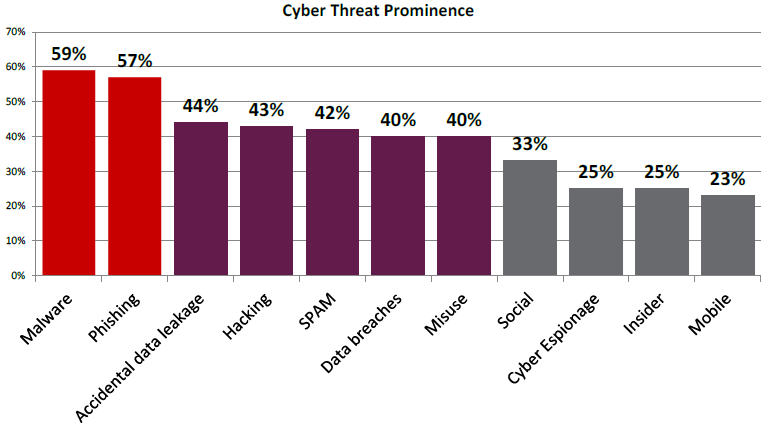
\includegraphics[scale=0.43]{img1}
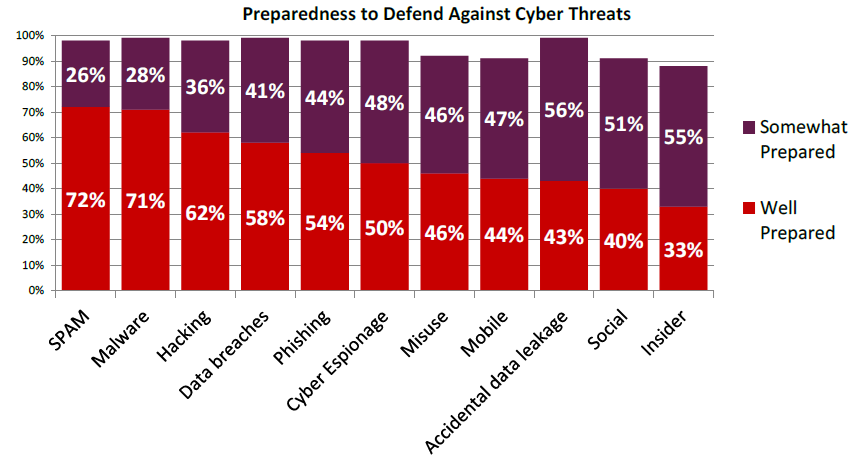
\includegraphics[scale=0.40]{img2}
\captionof{figure}{Proporción de cyber ataques (izquierda). Preparación ante cyber ataques (derecha)}
\end{center}
\underline{\textbf{Implementación}}
\begin{itemize}
\item Programa en R para limpieza de data.
\end{itemize}

}

%----------------------------------------------------------------------------------------
%	CONCLUSIONS
%----------------------------------------------------------------------------------------
\headerbox{Conclusiones}{name=conclusion,span=1,column=2,below=methods}{
\begin{itemize}
\item Hemos visto que Big Data es una de las más grandes tendencias hoy por hoy, pero que trae consigo nuevas, cada vez más numerosas y peligrosas amenazas.
\item Se mostró una implementación sencilla pero bastante ilustrativa sobre la limpieza de data, lo cual es necesario para realizar un buen y exitoso análisis.
\end{itemize}
}

%----------------------------------------------------------------------------------------
%	RESULTS
%----------------------------------------------------------------------------------------
\headerbox{Resultados}{name=results2,span=2,column=0,below=methods}{

%------------------------------------------------

\begin{center}
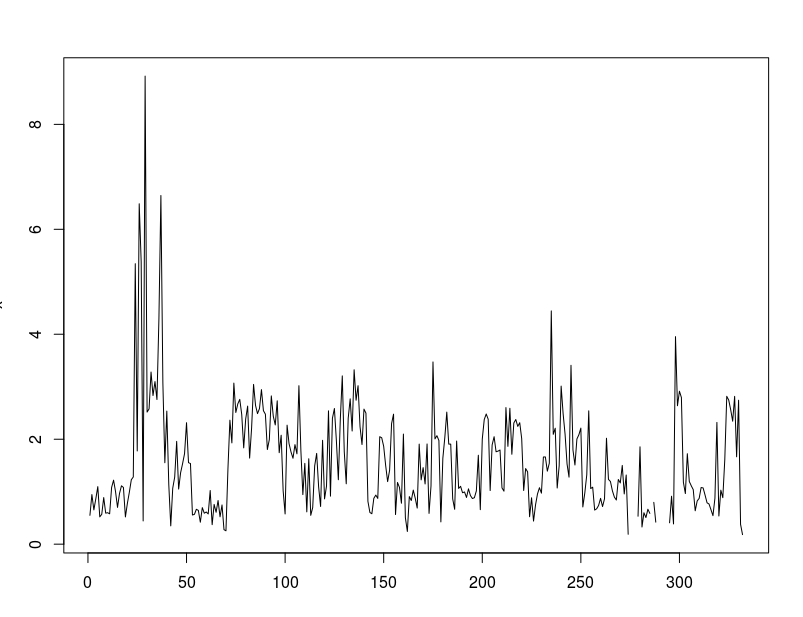
\includegraphics[width=0.55\linewidth]{nitrate}
\captionof{figure}{Concentración de nitrato}
\end{center}

\begin{center}
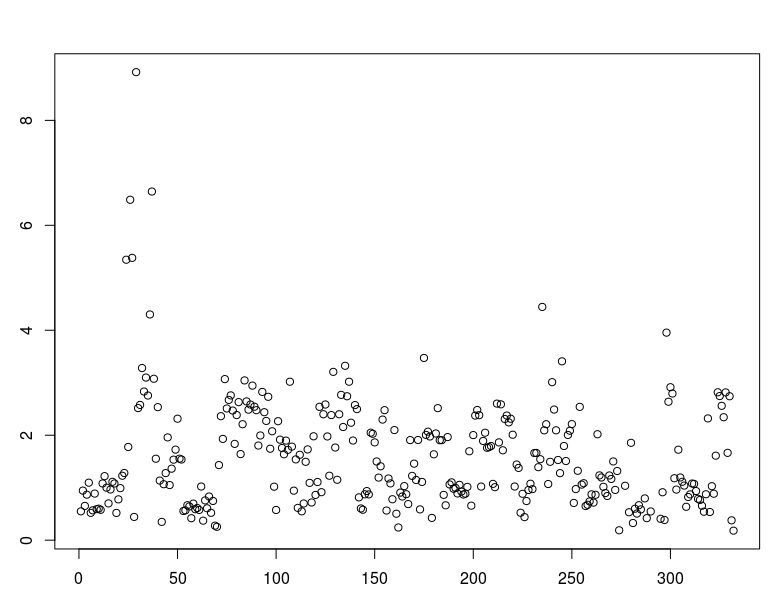
\includegraphics[width=0.55\linewidth]{sulfate}
\captionof{figure}{Concentración de sulfato}
\end{center}

%------------------------------------------------

}

%----------------------------------------------------------------------------------------
%	REFERENCES
%----------------------------------------------------------------------------------------
\headerbox{Referencias}{name=references,column=2, below=conclusion}{

\smaller % Reduce the font size in this block
\renewcommand{\section}[2]{\vskip 0.05em} % Get rid of the default "References" section title
\nocite{*} % Insert publications even if they are not cited in the poster
\begin{thebibliography}{1}
\bibitem{brid} Big data: The next frontier for innovation, competition, and productivity. James Manyika, Michael Chui, Brad Brown, Jacques Bughin, Richard Dobbs, Charles Roxburgh, and Angela Hung Byers. McKinsey Global Institute. May 2011.
\bibitem{par} Using Data for Systemic Financial Risk Management. Mark Flood, H V Jagadish, Albert Kyle, Frank Olken, and Louiqa Raschid. Proc. Fifth Biennial Conf. Innovative Data Systems Research, Jan. 2011.
\end{thebibliography}

}

%----------------------------------------------------------------------------------------

\end{poster}
\end{document}